
\chapter[Numerical Methods for the Advection Equation...]{Numerical
  Methods for the Advection Equation and Hyperbolic systems}\label{chap8}    

\section{Introduction}\label{chap8:sec8.1}

We now\pageoriginale study numerical schemes for the advection
equation which is a scalar equation. We consider the equation with
constant coefficients in order to apply Fourier transform techniques
to study stability. We do this for the pure initial value problems and
give modifications for problems with boundary conditions. Later we
shall extend these ideas to simple non-linear cases like Burger's
equation and also to systems of linear equations.  

The advection equation with constant coefficients is given by
\begin{equation*}
\frac{\partial u}{\partial t} + a \frac{\partial u}{\partial x} = 0.
\tag{8.1}\label{eq8.1}
\end{equation*}

To start with we establish a uniform mesh of step $\Delta x$ over
$\mathbb{R}$ and step $\Delta  t$ in time. As usual $u^n_i$ will
denote the value $u(i\Delta x, n \Delta t)$. We now proceed to give
various numerical schemes for the equation (\ref{eq8.1}). 

\section{Explicit Schemes for the Advection Equation}\label{chap8:sec8.2}

\begin{exam}\label{chap8:exam8.1}
The simplest shceme to approximate equation (\ref{eq8.1}) is given by
\begin{equation*}
\frac{u^{n+1}_i  - u^n_i}{\Delta t} + a \frac{u^n_{i+1} - u^n_{i-1}}{2 \Delta x} =0. 
\tag{8.2}\label{eq8.2}
\end{equation*}

It is obvious from expanding by a Taylor series about $(i \Delta x, \; n \Delta t)$ this scheme has an error of discretization of order $O(\Delta x^2 + \Delta t)$. However setting
\begin{equation*}
\alpha = a \frac{\Delta t}{\Delta x}\tag{8.3}\label{eq8.3}
\end{equation*}
and using the Fourier transform, the coefficient of amplification turns out to be 
\begin{equation*}
a (\xi) = 1 + i \alpha  \sin (\xi \Delta x).\tag{8.4}\label{eq8.4}
\end{equation*}\pageoriginale
Hence $|a (\xi)| \geq 1$, which means that this extremely simple explicit shceme is always unstable and is thus never used!
\end{exam}

\begin{exam}\label{chap8:exam8.2}
{\em Lax's Scheme}. This is an explicit scheme of first order accuracy, given by 
\begin{equation*}
\frac{u^{n+1}_i - \frac{1}{2} (u^n_{i+1} + u^n_{i-1})}{\Delta t} + a \frac{(u^n_{i+1} - u^n_{i-1})}{2 \Delta x} = 0. \tag{8.5}\label{eq8.5}
\end{equation*}

Again, from the Fourier transform, we get 
\begin{equation*}
a(\xi) = \Cos (\xi \Delta x) + i \alpha \sin (\xi \Delta x) \tag{8.6}\label{eq8.6}
\end{equation*}
where $\alpha$ is as in (\ref{eq8.3}). The criterion $|a(\xi)| \leq 1$ for all $\xi$, gives the stability condition, $|\alpha| \leq 1$, which is 
\begin{equation*}
|a| \frac{\Delta t}{\Delta x} \leq 1.\tag{8.7}\label{eq8.7}
\end{equation*}

This scheme has an error of discretization of order $O(\Delta x^2 + \Delta t + \dfrac{\Delta x^2}{\Delta t})$.
\end{exam}

\begin{exam}\label{chap8:exam8.3}
{\em One-sided scheme}. The scheme is defined by
\begin{equation*}
\frac{u^{n+1}_i - u^n_i}{\Delta t} + 
\begin{cases}
a \dfrac{(u^n_i - u^n_{i-1})}{\Delta x} = 0, \text{ if } a > 0\\
a \dfrac{(u^n_{i+1} - u^n_i)}{\Delta x} = 0, \text{ if } a < 0.
\end{cases}\tag{8.8}\label{eq8.8}
\end{equation*}

To motivate this, one can argue with characteristics. Assume that
$a>0$. Then the characteristics have positive slope. The value
$u^{n+1}_i$ is then the value at the point where the characteristic
through $(i\Delta x, (n+1)\Delta t) $ meets the level $n\Delta t$,
(Cf. Fig. 8.1) which we assume lies between $((i-1)\Delta x, n \Delta
t)$ and $((i+1) \Delta x, \; n \Delta t)$
(Cf. Remark \ref{chap8:rem8.2} on stability condition).  

\begin{figure}[H]
\centering
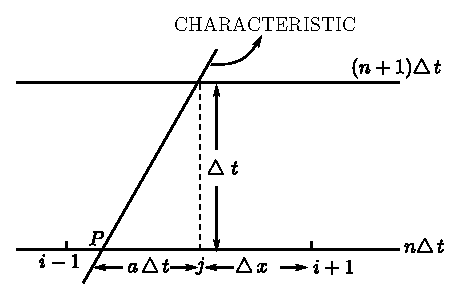
\includegraphics{figures/fig52-8.1.eps}
\caption{}\label{c8:fig8.1}
\end{figure}

To\pageoriginale get the value of $P$, we interpolate it linearly between the values $u^n_i$ and $u^n_{i-1}$. Writing this out we get precisely (\ref{eq8.8}) (multiplied throughour by $\Delta t$). Similarly we can treat the case $a < 0$.

This scheme has error of discretization of order $O(\Delta x + \Delta t)$. 
\end{exam}

\begin{exercise}\label{chap8:exer8.1}
Show that the stability condition (\ref{eq8.7}) holds in the case of the 1-sided scheme as well.
\end{exercise}

\begin{exam}\label{chap8:exam8.4}
{\em The Lax-Wendroff Scheme.} This is a second order scheme. We
motivate the scheme by the following arguments. Expanding $u^{n+1}_i$
by a Taylor expansion w.r.t. $t$, we get  
\begin{equation*}
  u^{n+1}_i = u^n_i + \Delta t \frac{\partial u}{\partial t} \big|^n_i +
  \frac{\Delta t^2}{2} \frac{\partial^2 u}{\partial t^2} \big|^n_i +
  \cdots .\tag{8.9}\label{eq8.9} 
\end{equation*}
Using the fact that $u$ satisfies the advection equation, we get 
\begin{align*}
\frac{\partial u }{\partial t} & = - a \frac{\partial u}{\partial x}\\
\frac{\partial^2 u}{\partial t^2} & = \frac{\partial}{\partial t } \left(-a
\frac{\partial u}{\partial x}\right) = a^2 \frac{\partial^2 u}{\partial
  x^2}. 
\end{align*}
Substituting, we get
\begin{equation*}
u^{n+1}_i = u^n_i  - a \Delta t \frac{\partial u}{\partial x}
\big|^n_i + a^2 \frac{\Delta t^2}{2} \frac{\partial^2 u}{\partial x^2}
\big|^n_i + \cdots  
\tag{8.10}\label{eq8.10} 
\end{equation*}\pageoriginale
We use (\ref{eq8.10}) as the guideline for forming the scheme which is given by 
$$
u^{n+1}_i = u^n_i - a \Delta t \frac{(u^n_{i+1} - u^n_{i-1})}{2\Delta
  t} + \frac{a^2 \Delta t^2}{2\Delta x^2} (u^n_{i-1} - 2u^n_i +
u^n_{i-1}).  
$$
Equivalently, we can write 
\begin{equation*}
\frac{u^{n+1}_i - u^n_i}{\Delta t} + a \frac{(u^n_{i+1} -
  u^n_{i-1})}{2\Delta x}  - \frac{a^2 \Delta t}{2\Delta x^2}
(u^n_{i+1} - 2u^n_i + u^n_{i-1}) = 0 
\tag{8.11}\label{eq8.11}
\end{equation*}

The error of discretization is of order $O(\Delta x^2 + \Delta t^2)$. 
\end{exam}

\begin{exercise}\label{chap8:exer8.2}
Find the coefficient of amplification $a(\xi)$ for the Lax-Wen\-droff
scheme and show that the stabilitity condition is again given by
(\ref{eq8.7}). 
\end{exercise}

\begin{remark}\label{chap8:rem8.1}
We may rewrite the scheme of Lax and the one-sided scheme as follows:

\medskip
\noindent{\textbf{Lax's shceme:}}
\begin{equation*}
\frac{u^{n+1}_i - u^n_i}{\Delta t} +  a\frac{(u^n_{i+1} -
  u^n_{i-1})}{2\Delta x} - \frac{\Delta x^2}{2 \Delta t}
\left(\frac{u^n_{i+1} - 2u^n_i + u^n_{i-1}}{\Delta x^2}\right) =0 
\tag{8.12}\label{eq8.12}
\end{equation*}

\medskip
\noindent{\textbf{One-Sided scheme:}}
\begin{equation*}
\frac{u^{n+1}_i - u^n_i}{\Delta t} + a \frac{(u^n_{i+1} -
  u^n_{i-1})}{2\Delta x} -\frac{|a|\Delta x}{2} \left(\frac{u^n_{i+1} -
  2u^n_i + u^n_{i-1}}{\Delta x^2}\right) = 0 \tag{8.13}\label{eq8.13}
\end{equation*}

In writing both (\ref{eq8.12}) and (\ref{eq8.13}) we see that we have essentially approximated to second order accuracy, the perturbed equation
\begin{equation*}
\frac{\partial u}{\partial t} + \frac{\Delta t }{2} \frac{\partial^2
  u}{\partial t^2} + a \frac{\partial u}{\partial x} - \epsilon
\frac{\partial^2 u}{\partial x^2} = 0.\tag{8.14}\label{eq8.14} 
\end{equation*}
where $\epsilon$ is the coefficient occuring in the last term of
(\ref{eq8.12}) or (\ref{eq8.13}). Since the solution\pageoriginale
satisfies (\ref{eq8.1}), we can rewrite (\ref{eq8.14}) as  
\begin{equation*}
\frac{\partial u}{\partial t} + a  \frac{\partial u}{\partial x} -
\left(\epsilon - \frac{a^2 \Delta t}{2}\right) \frac{\partial^2 u}{\partial x^2}
= 0. 
\tag*{$(8.14)'$}\label{eq8.14'} 
\end{equation*}
A criterion of stability due to Hirt \cite{key15}  and Yanenko is the
$\epsilon - \dfrac{a^2 \Delta t}{2} \geq 0$. This last term involving
$\epsilon$ is called the dissipative term. In all cases $\epsilon \to
0$ as $\Delta x$, $\Delta t \to 0$ (and, if $\dfrac{\Delta x^2}{\Delta
  t} \to 0$ in case of Lax's scheme). 
\end{remark}

\begin{remark}\label{chap8:rem8.2}
{\em Interpretations with characteristics}. Just as the one-sided
scheme was interpreted to be a linear interpolation between $x_{i+1}$
and $x_i(a<0)$ or between $x_i$ and $x_{i-1}(a>0)$, we can interpret
the Lax scheme as linear interpolation between $x_{i+1}$ and
$x_{i-1}$. The Lax-Wendroff scheme is the quadratic interpolation
between $x_{i+1}, x_i$ and $x_{i-1}$. All these three interpolations
are for the same point $P$ of Fig. \ref{c8:fig8.1}. 

We may also interpret the stability condition in terms of characteristics.

Consider the mesh given in Fig. \ref{c8:fig8.2}.

\begin{figure}[H]
\centering
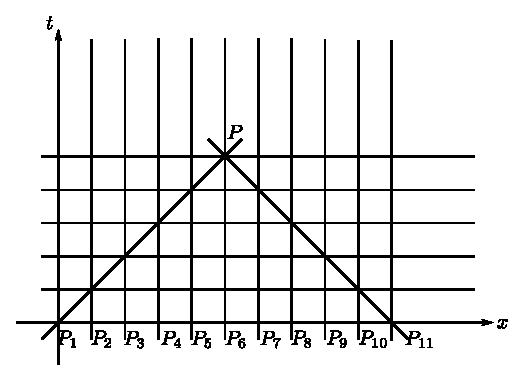
\includegraphics{figures/fig52-8.2.eps}
\caption{}\label{c8:fig8.2}
\end{figure}

The\pageoriginale stability condition implies that $\Delta t$ cannot
be too large compared to $\Delta x$.  Note that for the approximate
schemes given above the value at $P$ depends on the values on the 3
nodes immediately below and they in terms of the 5 nodes below them
and so on. Thus we define the approximate domain of dependence for $P$
at any time level to be that portion of the grid between $P_1 P$ and
$P_{11} P $. However, if the stability condition is violated, then the
characteristic through $P$ will lie outside the region between these
two lines and the exact domain of dependence, which is a single point
for the advection equation, (if $P= (x,t)$ then the exact domain of
dependence at $t=0$ is the point $(x- ut, 0)$, Cf. 1.6), will lie
outside this region. This will violate the Courant-Friedrichs-Lewy
convergence condition that {\em the exact domain of dependence must be
  contained in the approximate domain of } dependence and we will not
get convergence when $\Delta x$, $\Delta t \to 0$ keeping
$\dfrac{\Delta t}{\Delta x}$ constant. 
\end{remark}

\section{Implicit Schemes for the Advection
  Equation}\label{chap8:sec8.3}

We will now look at a few implicit schemes for the advection equation.

\begin{exam}\label{chap8:exam8.5}
{\em The SNG-Scheme}. This scheme was devised by Carlson for the
neutron transport equation. It is a method of first order of accuracy
and is essentially an extension of the oen-sided scheme. 

Let us assume $a>0$. (The details when $a <0$ follow a parallel line
of thought). 

When $\dfrac{a \Delta t}{\Delta x} \leq 1$, one uses the one-sided scheme which was only a linear interpolation between the points $i$ and $i+1$ at time $n \Delta t$. 

If $\dfrac{a\Delta t}{\Delta x} > 1$, then the characteristic through
($i\Delta x$, $(n+1)\Delta t$) meets the line $x = (i-1)\Delta x$
before it meets $t = n \Delta t$ (See Fig. \ref{c8:fig8.3}).  

\begin{figure}[H]
\centering{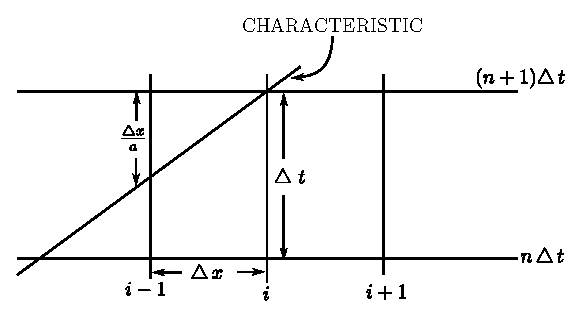
\includegraphics{figures/fig52-8.3.eps}}
\caption{}\label{c8:fig8.3}
\end{figure}

Hence\pageoriginale we now have the value  $u^{n+1}_i$ equal to the
value of $u$ at $P$ which we interpolate linearly between $((i-1)
\Delta x, \; n \Delta t)$ and $((i-1)\Delta x, \; (n+1)\Delta t)$, to
get 
$$
u^{n+1}_i = (1 - \frac{\Delta x}{a \Delta t}) u^{n+1}_{i-1} +
\frac{\Delta x}{a\Delta t} u^n_{i-1} 
$$
or equivalently,
\begin{equation*}
\frac{u^{n+1}_{i-1} - u^n_{i-1}}{\Delta t} + a \frac{(u^{n+1}_i -
  u^{n+1}_{i-1})}{\Delta x}  = 0\tag{8.15}\label{eq8.15} 
\end{equation*}

The SNG scheme consists of (\ref{eq8.15}) as well as the one-sided scheme depending on the value of $\alpha = \dfrac{a\Delta t}{\Delta x}$. In case of (\ref{eq8.15}) being used one has
\begin{equation*}
a (\xi) = (1+ \alpha (e^{-i\xi \Delta x} -1))^{-1}\tag{8.16}\label{eq8.16}
\end{equation*}
and $|a(\xi)| \leq 1$ if $\alpha >1$, which is indeed true. Thus the scheme is {\em unconditionally stable}.

Suppose we have to work in a bounded interval, say, $0 < x< 1$. Then, when $a>0$, one can impose a boundary condition on $x=0$. 

\begin{figure}[H]
\centering
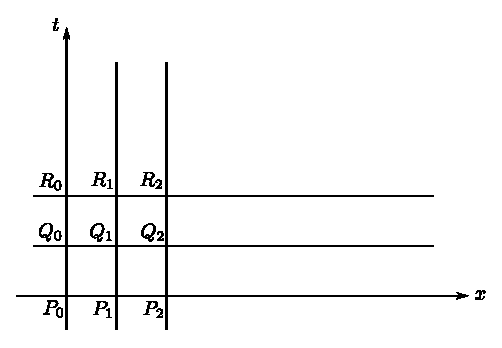
\includegraphics{figures/fig52-8.4.eps}
\caption{}\label{c8:fig8.4}
\end{figure}

Then to\pageoriginale calculate $Q_1$, we know the values at $Q_\circ$, $P_\circ$ and $P_1$ and hence the value at $Q_1$ can be calculated explicitly from the scheme. Now for $Q_2$, since we know the values at $Q_1 , P_1$ and $P_2$, we can calculate the value at $Q_2$ and so on. This can be done at any level $n \Delta t$. Thus though the scheme is {\em formally implicit}, one can, with the aid of the initial value and the boundary condition, solve for the value at each node {\em explicitly, step by step}. Such a scheme is called quasiexplicit. 
\end{exam}

\begin{remark}\label{chap8:rem8.3}
In case of the neutron transport equation, one has to solve the
equation (\ref{eq8.1}) when a take its values over an interval
$[-A,A]$, using the {\em same } time step $\Delta t$  for all $a$ in
this interval. Hence it is here that the SNG scheme is very useful, it
being unconditionally stable. 
\end{remark}

\begin{exam}\label{chap8:exam8.6}
{\em The Crank-Nicolson Scheme}. The scheme is given by 
\begin{equation*}
\frac{u^{n+1}_i - u^n_i}{\Delta t} + \frac{a}{2} \left[\frac{u^{n+1}_{i+1} - u^{n+1}_{i-1}}{2\Delta x} + \frac{u^n_{i+1} - u^n_{i-1}}{2\Delta x} \right] = 0
\tag{8.17}\label{eq8.17}
\end{equation*}
This scheme is of second order and is also unconditionally
stable. However, it is purely\pageoriginale an implicit scheme unlike the
SNG-scheme. 

In this linear case, this leads to a system with a tridiagonal matrix which is easy to solve by Gauss' method adapted to a tridiagonal system. But in using this scheme for the non-linear equation, with $u$'s in the second term of (\ref{eq8.17}) being replaced by a function $f(u)$, the solution becomes more complicated. Thus one devises iterative methods. Let $u^{n,p}_i$ denote the value of $u^n_i$ at the $p^{\rm th}$-iteration. We can use then the following methods.
$$
\frac{u^{n+1, p+1}_i - u^n_i }{\Delta t} + \frac{a}{2} \left[  \frac{u^{n+1, p}_{i+1} - u^{n-1,p}_{i-1}}{2\Delta x} + \frac{u^n_{i+1} - u^n_{i-1}}{2\Delta x}\right] = 0
$$
where we assume all values $u^n_i$ to be known. If $U^T = (u^{n+1}_1 , \ldots u^{n+1}_1)$, we get
\begin{equation*}
U^{(p+1)} = - \frac{a\Delta t}{4\Delta x} 
\begin{pmatrix}
0 & 1 & 0 & \cdot & \cdot & \cdot & 0\\
-1 & 0 & 1 & \cdot & \cdot & \cdot & 0\\
\cdot & \cdot & \cdot & \cdot & \cdot & \cdot & \cdot \\
\cdot & \cdot & \cdot & \cdot & -1 & 0 & 1\\ 
\cdot & \cdot & \cdot & \cdot & 0 & -1 & 0
\end{pmatrix} U^{(p)} + F
\tag{8.18}\label{eq8.18}
\end{equation*}
where $F$ is known. The convergence of this iterative method implies and is implied by $\rho (H) <1$, where $H$ is the matrix occurring as the coefficient of $U^{(p)}$ in (\ref{eq8.18}). Here $\rho (H) \sim \dfrac{|a|}{2} \dfrac{\Delta t}{\Delta x}$.  Thus in the non-linear case we have to resort to an iterative method which ends up with a condition similar to the stability condition and this undoes all our advantages of achieving unconditional stability.

Of course, one can devise better iterative methods but considerations
like computer time etc. do not make this worthwhile. If to solve the
Crank-Nicolson scheme with $a \Delta t$, $N$ times larger than the
time step allowed for an explicit scheme $\left(\Delta t < \dfrac{\Delta
  x}{|a|}\right)$ one needs $M>N$ iterations, then obviously the scheme is
not worthwhile. Moreover consideration of accuracy usually prohibits
taking $\Delta t$ large compared to $\dfrac{\Delta x}{|a|}$. 
\end{exam}

\begin{exam}\label{chap8:exam8.7}
This\pageoriginale scheme was used by Robert and Weiss \cite{key34} in
fluid dynamics. The scheme is of second order accuracy and is
quasi-explicit when we have a boundary condition. It is also
unconditionally stable. (Exercise: check these assertions!) To put
down the scheme, we approximate the derivative w.r.t. $x$ by using the
mid-points of the diagonals, shown in Fig. \ref{c8:fig8.5}. when $a>0$. 

\begin{figure}[H]
\centering
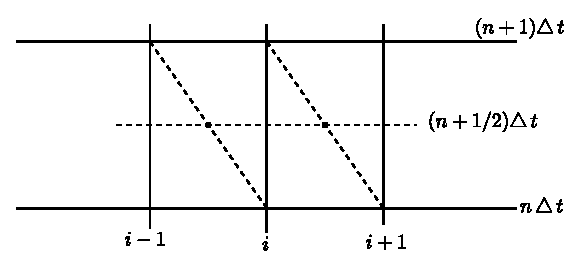
\includegraphics{figures/fig52-8.5.eps}
\caption{}\label{c8:fig8.5}
\end{figure}
\begin{equation*}
\frac{u^{n+1}_i - u^n_i}{\Delta t} + \frac{a}{\Delta x} \left[\frac{u^{n+1}_i + u^n_{i+1}}{2} - \frac{u^{n+1}_{i-1} + u^n_i}{2} \right] = 0.\tag{8.19}\label{eq8.19}
\end{equation*}
when $a>0$.

If $a<0$, we use the other two diagonals of these rectangles. This scheme is rarely used.
\end{exam}

\begin{exam}\label{chap8:exam8.8}
{\em The DSN--Scheme}. This was also devised by Carlson for the neutron transport equation. In each rectangle of the grid, one evaluates the values of $u$ at the four mid-points of the sides and at the centroid.

\begin{figure}[H]
\centering
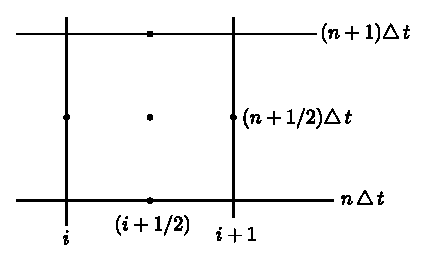
\includegraphics{figures/fig52-8.6.eps}
\caption{}\label{c8:fig8.6}
\end{figure}

For\pageoriginale this we use the set of three equations given below:
\begin{equation*}
\begin{cases}
{\rm (i)}  \qquad & \dfrac{u^{n+1}_{i+\frac{1}{2}} - u^n_{i+\frac{1}{2}}}{\Delta t} + a \dfrac{(u^{n+\frac{1}{2}}_{i+1} - u^{n+\frac{1}{2}}_i)}{\Delta x} = 0,\\[6pt] 
{\rm (ii)} \qquad &  2u^{n+\frac{1}{2}}_{i+\frac{1}{2}} = u^{n+1}_{i+\frac{1}{2}} + u^n_{i+\frac{1}{2}} = u^{n+\frac{1}{2}}_{i+1} + u^{n+\frac{1}{2}}_i 
\end{cases}
\tag{8.20}\label{eq8.20}
\end{equation*}

This scheme is quasi explicit for the following reasons. (our
notations are based on Fig. \ref{c8:fig8.7}). 

\begin{figure}[H]
\centering
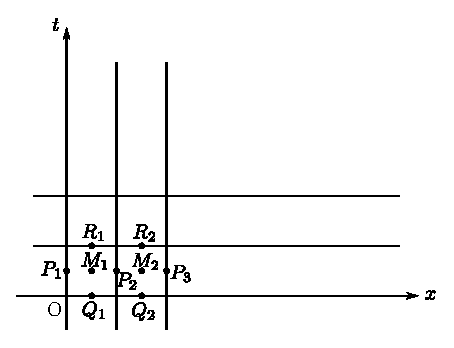
\includegraphics{figures/fig52-8.7.eps}
\caption{}\label{c8:fig8.7}
\end{figure}

Assume $a>0$. We then can have a boundary condition on $x=0$. Hence
from the boundary and initial conditions, we know the values of $u$ at
$P_1$ and $Q_1$. 
Using\pageoriginale equations (\ref{eq8.20}) (ii) we can express the
values at $R_1$ and $P_2$ in terms of that at $M_1$. Now
(\ref{eq8.20}) (i) reduces to an equation in one unknown, viz., the
value at $M_1$ and we can solve for this explicitly and from this get
back the values at $R_1$ and $P_2$. 

Thus step by step we can evaluate, explicitly, all the unknowns. The
scheme is therefore quasi-explicit. The scheme is of second order
accuracy. However, for the stability one cannot use the Fourier
transform. But one can get an energy inequality and we leave this as
an exercise. 
\end{exam}

\begin{exercise}\label{chap8:exer8.3}
Using an energy inequality show that the DSN-scheme is unconditionally
stable. 
\end{exercise}


\section{Comparison of the Schemes Above}\label{chap8:sec8.4}

We summarize the main features of the preceding schemes in table 8.1.

\newpage

\rotatebox{90}{
{\fontsize{8}{10}\selectfont
\begin{tabular}{llllll}
\hline
& & & & Possibility & \\
Type & Name of the & $(L^2)$ Stabi- & Order of & of extension & Comments\\
& scheme & lity & accuracy & to systems & \\
\hline
Explicit & Centred & Always un- & {~\quad -}  &  {~\quad - } & Never used\\
& scheme. & stable & & &  \\[5pt]
 & Lax's & $|a|\dfrac{\Delta t}{\Delta x} \leq 1$ for & {~\quad 1} & {~\quad Yes }
&  \multirow{3}{2cm}{$L^\infty$-stable as well}\\
& Scheme. &  stability & & &\\[5pt]
& One-sided & \multirow{2}{1cm}{~ \quad $''$} & \multirow{2}{1cm}{~\quad 1} & \multirow{2}{1cm}{~\quad No} & \\
& scheme & & & & \\[5pt]
& Lax-Wendroff & \multirow{2}{1cm}{~ \quad $''$} &
\multirow{2}{1cm}{~\quad 2} & \multirow{2}{1cm}{~\quad Yes} & This
is the best\\ 
& scheme. & & &  & among the \\
& & & & & explicit schemes.\\
& & & & &  But it is not\\
& & & & &  $L^\infty$-stable.\\
\hline
\multirow{2}{1cm}{Implicit} & Crank-Nicolson &  Unconditionally &
\multirow{2}{1cm}{~\quad 2} & \multirow{2}{1cm}{~\quad  Yes} &
\multirow{2}{1.5cm}{Rarely used}\\ 
& scheme & stable & & & 
\\
\hline
Quasi- & SNG-Scheme & {~\quad $''$} & {~\quad 1} & By method of & Used for neutron\\
explicit & & &  & characteristics & transport equation\\[5pt]
& DSN-Scheme & {~\quad $''$} & {~\quad 2} & Yes, but exten- & \multirow{3}{1cm}{~\qquad $''$}\\
& & & & sion is purely & \\
& & & & implicit & \\
& Robert-Weiss' & \multirow{2}{1cm}{~\quad $''$} &  & \multirow{2}{1.5cm}{Rarely used}\\
& scheme & & & & \\
\hline
\end{tabular}}}
\pageoriginale

\newpage

\begin{remark}\label{chap8:rem8.4}
As mentioned in Table 8.1, the Lax-Wendroff scheme is not
$L^\infty$-stable. (Cf. Them\'ee \cite{key36}). If the initial value
of the solution of the advection equation has a shock, so has $u(x,t)$
for any time $t$. If one uses the Lax-Wendroff scheme, the approximate
solution has a lot of oscillations about such a discontinuity. This
behaviour is related to the $L^\infty$-instability of the scheme. The
Lax and the one-sided scheme, on the other hand, are $L^\infty$-stable
but their approximate solutions are too smooth around the point of
discontinuity of the true solution and this does not represent the
ture situation either. In practice one has to exercise one's own
judgement as to which behaviour is preferable! One can also add a
non-linear dissipative term to the equation (\ref{eq8.1}) which is
negligible everywhere except at a shock where it has to smooth out the
oscillations. See Boris and Book \cite{key4} and Van de Leer
\cite{key37}. 
\end{remark}

\section{The non-linear equations}\label{chap8:sec8.5}
The non-linear equation takes the form
\begin{equation*}
\frac{\partial u}{\partial t} + \frac{\partial}{\partial x} (f(u)) = 0.
\tag{8.21}\label{eq8.21}
\end{equation*}

If one wants to imitate the Lax-Wendroff scheme, one again motivates this by the Taylor expansion:
\begin{align*}
u^{n+1} & = u^n + \Delta t u_t + \frac{\Delta t^2}{2} u_{tt} + \ldots \\
& = u^n - \Delta t (f(u))_x + \frac{\Delta t^2}{2} \frac{\partial
}{\partial x} \left(f'(u) \frac{\partial f(u)}{\partial x}\right)  + \ldots  
\end{align*}\pageoriginale
again using (\ref{eq8.21}). In case of a non-linear {\em system}, the
matrix $f'(u)$ might be very difficult to compute. Hence one modifies
the Lax - Wendroff scheme to avoid this difficulty and permit
generalization to systems. This is called the {\em 2-step Lax-Wendroff
  scheme} which is described as follows: 

\medskip
\noindent{\textbf{Step I.}}
 Using $u^n_{i+1}$ and $u^n_i$, one obtains, say, by the Lax's scheme, $u^{n+\frac{1}{2}}_{i-\frac{1}{2}}$. Using $u^n_i$, $u^n_{i-1}$ one obtains  $u^{n+\frac{1}{2}}_{i-\frac{1}{2}}$ in the same fashion.

\medskip
\noindent{\textbf{Step II.}}
Using the results of step I, we write the scheme
\begin{equation*}
\frac{u^{n+1}_i - u^n_i}{\Delta t} +
\frac{f\left(u^{n+\frac{1}{2}}_{i-\frac{1}{2}}\right) -
  f\left(u^{n+\frac{1}{2}}_{i-\frac{1}{2}}\right) }{\Delta x}=
0.\tag{8.22}\label{eq8.22} 
\end{equation*}

In the linear case when $f(u) = au$, this reduces to the usual Lax-Wendroff scheme (check!).

The scheme we have just described is a memeber of class of schemes known as $S^\beta_\alpha$-schemes, all of which reduce to the Lax-Wendroff scheme in the linear case. These have been studied by Lerat and Peyret \cite{key25}.

All these schemes give oscillations about a shock. To treat this we can add a dissipative term to the differential equation so that this term is small where the gradient of the solution is small and acts only where the gradient is large i.e. at a shock. One such term is the pseudo-viscosity term and in this case the equation reads as
\begin{equation*}
\frac{\partial u}{\partial t} + \frac{\partial }{\partial x} (f(u)) -
\epsilon \frac{\partial }{\partial x} \left(|\frac{\partial f'(u)}{\partial
  x}| \frac{\partial u}{\partial x}\right) =0. \tag{8.23}\label{eq8.23} 
\end{equation*}

One uses the Lax-Wendroff scheme for the first two terms and add an explicit\pageoriginale approximation to the dissipative term.

There is no rigorous rule for the choice of the dissipative term. However, one can apply a dimension analysis to get some idea about it.

Raviart \cite{key31} has studied the convergence when $\Delta x$, $\Delta t \to 0$ of three schemes for the equation (\ref{eq8.23}) with $f(u) = \frac{1}{2} u^2$, but with $\epsilon$ fixed. This of course, is not exactly the state of affairs since we require $\epsilon$ to be small and $\to 0$. How ever, this is a step in the right direction.

\section{Boundary conditions}\label{chap8:sec8.6}
Let us consider the following problem with boundary conditions:
\begin{equation*}
\left.
\begin{aligned}
& \dfrac{\partial u}{\partial t} +  a \dfrac{\partial u}{\partial x} =
  0, \quad a > 0, \quad 0 < x < 1\\ 
& u(x,0) = u_\circ (x), \text{ (initial value)}\\
& u(0, t) = 0 \text{ (boundary value)}
\end{aligned}
\right\}\tag{8.24}\label{eq8.24}
\end{equation*}

We have seen that when there is no condition on $x=1$, this problem is well posed. (Cf. Sec. \ref{chap5:sec5.3}).

The various numerical schemes cited for the purely initial-value
problems are all three point schemes involving $i-1$, $i$ and $i+1$ of
the previous level. However, in case of the bounded domain, if $0 \leq
i  \leq I$, then the equation for $u^{n+1}_I$ will involve $u^n_{I+1}$
which lies outside the domain and hence we do not know it. Thus one
feels the need for extrapolating $u^n$ to the point $I+1$ as well. One
such interpolation is provided by  
\begin{equation*}
u_{I+1} = u_I.\tag{8.25}\label{eq8.25}
\end{equation*}

However, this is not a sufficiently accurate choice. A much better choice 
\begin{equation*}
u_{I+1} = 2u_I - u_{I-1}.\tag{8.26}\label{eq8.26}
\end{equation*}\pageoriginale

One could, of course, give better extrapolation formulae, but as all schemes are of atmost second order accuracy, the formula (\ref{eq8.26}) is quite sufficient for our purposes.

\begin{exercise}\label{chap8:exer8.4}
Apply the formulae (\ref{eq8.25}) and (\ref{eq8.26}) to the Lax-Wendroff scheme and show that (\ref{eq8.25}) gives an inconsistent scheme while that given by (\ref{eq8.26}) is consistent.
\end{exercise}

\begin{remark}\label{chap8:rem8.5}
The stability of problems with boundary conditions is usually studied by the energy method. This problem has been studied deeply by kreiss \cite{key19}.
\end{remark}

\section{The leap-frog scheme}\label{chap8:sec8.7}
This scheme is given by
\begin{equation*}
\frac{u^{n+1}_i - u^{n-1}_i}{2\Delta t}  + a \frac{(u^n_{i+1} - u^n_{i-1})}{2\Delta x} = 0. \tag{8.27} \label{eq8.27}
\end{equation*}

This is a 3-level scheme which, though not widely used for the advection equation, is very useful for systems of hyperbolic equations, especially for the wave equation. It is easy to see that the scheme has an error of discretization, of order $O(\Delta x^2 + \Delta t^2)$ and hence is of second order of accuracy.

Setting $v^n_i = u^{n-1}_i$, we get the system
$$
\begin{bmatrix}
u^{n+1}_i\\
v^{n+1}_i
\end{bmatrix} = 
\begin{bmatrix}
\alpha & 0\\
0 & 0
\end{bmatrix}
\begin{bmatrix}
u^n_{i-1}\\ v^n_{i-1}
\end{bmatrix}
+
\begin{bmatrix}
0 & 1\\
1 & 0
\end{bmatrix}
\begin{bmatrix}
u^n_i \\ v^n_i
\end{bmatrix}
+
\begin{bmatrix}
-\alpha & 0\\
0 & 0
\end{bmatrix}
\begin{bmatrix}
u^n_{i+1} \\ v^n_{i+1}
\end{bmatrix}
$$
which gives 
$$
\begin{bmatrix}
\hat{u}^{n+1}(\xi)\\
\hat{v}^{n+1}(\xi)
\end{bmatrix}
=
\begin{bmatrix}
2iA & 1 \\
1 & 0
\end{bmatrix}
\begin{bmatrix}
\hat{u}^n (\xi)\\
\hat{v}^n (\xi)
\end{bmatrix}
$$
where\pageoriginale $A = a\dfrac{\Delta t}{\Delta x} \sin\xi \Delta x$.

The eigenvalues are given by the roots of the equation 
$$
\lambda^2 - 2i A \lambda - 1 = 0.
$$
If $1-A^2 \geq 0$, then 
$$
\lambda = i A \pm \sqrt{1-A}^2
$$
and if $1-A^2 \leq 0$, then 
$$
\lambda = i A \pm i \sqrt{A^2 -1}
$$

In the latter case $|\lambda |>1$ for at least one $\lambda$ and in the former case $|\lambda| =1$ for both eigen values. Thus we get the stability condition $|A| \leq 1$ for all $\xi$, which is the condition
\begin{equation*}
|a| \frac{\Delta t}{\Delta x} \leq 1. \tag{8.28}\label{eq8.28}
\end{equation*}
Note that this condition is {\em necessary}.

We can get a {\em sufficient} condition if the matrix of amplification is diagonalizable. Let
$$
A(\xi) = S(\xi) D(\xi) S^{-1} (\xi). 
$$
Then $A^n(\xi) = SD^n S^{-1} (\xi)$. By the preceding necessary condition for stability, one has $||D^n||$ bounded. Thus a sufficient condition is 
\begin{equation*}
\max\limits_{\xi} (||S(\xi)|| + ||S^{-1} (\xi)||)  \leq \text{ constant}. \tag{8.29} \label{eq8.29}
\end{equation*}

Applying this to the Leap-frong scheme, if $\alpha = |a| \dfrac{\Delta t}{\Delta x} < 1$, then $|A|^2 < 1$ and the eigenvalues are distinct. The sufficient condition (\ref{eq8.29}) is indeed satisfied. (Check!).

On the other hand, if $\alpha =1$ and $\xi \Delta x = \pi/2$, then $\lambda_1 = \lambda_2$ and $A$ is not diagonalizable. Thus the sufficient condition is not satisfied. Though this is no proof\pageoriginale of instability, we give below an example of this situation where the scheme is indeed unstable.

\begin{exercise}\label{chap8:exer8.5}
In the leap-frog scheme with $\alpha =1$, given $u^\circ_j = \exp
\left(\dfrac{i\pi j}{2}\right)$ and $u^1_j = \exp
\left(\dfrac{i\pi(j+1)}{2}\right)$, show that 
$$
u^n_j = (2n-1) \exp. \left(\frac{i\pi}{2} (j+2 - n)\right), \quad n \geq 1,
$$
and hence the scheme is unstable.
\end{exercise}

Finally, when dealing with bounded domains, we need to extrapolate at the point $I+1$, where $0 \leq i \leq I$  are the nodes of the mesh. The following procedure of extrapolation can be proved (by the energy method) to be stable although it is probably not the best one w.r.t. accuracy:
\begin{equation*}
u^n_{I+1} = \frac{1}{2} (u^{n+1}_I + u^{n-1}_I). \tag{8.30}\label{eq8.30}
\end{equation*}

One can show, by energy methods, the stability of the scheme under the sufficient condition
\begin{equation*}
|a| \frac{\Delta t}{\Delta x} < 1. \tag{8.31}\label{eq8.31}
\end{equation*}

We demonstrate this when the domain is $\mathbb{R}$ and leave the boundary condition case as an exercise.

Multiplying the equation (\ref{eq8.27}) by $\Delta x (u^{n+1}_i + u^{n-1}_i)$ and summing over all $i$, we get 
\begin{equation*}
\frac{|u^{n+1}|^2 - |u^{n-1}|^2}{2\Delta t} + \frac{a}{2}
\left(\sum\limits_i (u^n_{i+1} - u^n_{i-1}) u^{n+1}_i + \sum\limits_i
(u^n_{i+1} - u^n_{i-1}) u^{n-1}_i\right) = 0, \tag{8.32}\label{eq8.32} 
\end{equation*}
where $|\cdot |$ is the $\ell^2$-norm induced by the innerproduct defined in sec. \ref{chap7:sec7.6} (Cf. equation \ref{eq7.18}). Now, one can easily verify that the following holds (by a simple)
\begin{equation*}
\sum\limits_i (u^n_{i+1} - u^n_{i-1})u^{n-1}_i = - \sum\limits_i (u^{n-1}_{i+1} - u^{n-1}_{i-1}) u^n_i. \tag{8.33}\label{eq8.33}
\end{equation*}\pageoriginale
We now define
\begin{equation*}
X^{n+\frac{1}{2}} = |u^{n+1}|^2 + |u^n|^2 + \frac{a\Delta t}{\Delta x} \cdot \Delta x \sum\limits_i (u^n_{i+1} - u^n_{i-1}) u^{n+1}_i. \tag{8.34}\label{eq8.34}
\end{equation*}
Using (\ref{eq8.33}) and (\ref{eq8.34}), (\ref{eq8.32}) becomes
$$
X^{n+\frac{1}{2}} = X^{n-\frac{1}{2}}.
$$
Proceeding recursively, one gets
\begin{equation*}
X^{n+\frac{1}{2}} = X^{n-\frac{1}{2}} = \ldots = X^{\frac{1}{2}}. 
\tag{8.35}\label{eq8.35}
\end{equation*}

Note that $X^{\frac{1}{2}}$ is expressed in terms of $u^\circ$ and $u^1$ and hence is known. Further $X^{n+\frac{1}{2}}$ is bounded.

Observe that 
\begin{align*}
|\Delta x \sum\limits_i (u^n_{i+1} - u^n_{i-1}) u^{n+1}_i| &  \leq \sqrt{\Delta x \sum\limits_i |u^n_{i+1} - u^n_{i-1}|^2 \cdot |u^{n+1}|}\\
& \leq 2 |u^n| \cdot |u^{n+1}|\\
& \leq |u^n|^2 + |u^{n+1}|^2,
\end{align*}
by using the Cauchy-Schwarz and the Minkowski inequalities for the innerproduct and norm respectively and also the fact that non-negative $a$ and $b$, $2ab \leq a^2 + b^2$. Thus
\begin{align*}
|X^{n+\frac{1}{2}}|& \leq |u^{n+1}|^2 + |u^n|^2 + |\alpha| (|u^{n+1}|^2 + |u^n|^2)\\
& = (1+|\alpha|) (|u^{n+1}|^2 + |u^n|^2) .
\end{align*}
Also
$$
|X^{n+\frac{1}{2}}| \geq |(|u^{n+1}|^2 + |u^n|^2) - |\alpha| \; | \Delta x \sum\limits_i (u^n_{i+1} - u^n_{i-1}) u^{n+1}_i ||
$$
But\pageoriginale
\begin{align*} 
& |u^{n+1}|^2 + |u^n|^2 - |\alpha| | \Delta x \sum\limits_i (u^n_{i+1} - u^n_{i-1}) u^{n+1}_i |\\
& \geq |u^{n+1}|^2 + |u^n|^2 - |\alpha| (|u^{n+1}|^2 + |u^n|^2)\\
& = (1-|\alpha|) (|u^{n+1}|^2 + |u^n|^2) \geq 0 \text{ if } |\alpha| \leq 1. 
\end{align*}
Thus one has 
\begin{equation*}
(1-|\alpha|) (|u^{n+1}|^2 + |u^n|^2) \leq |X^{n+\frac{1}{2}}| \leq ( 1+|\alpha|) (|u^{n+1}|^2 + |u^n|^2). \tag{8.36}\label{eq8.36}
\end{equation*}
If $|\alpha| <1$ (as in (\ref{eq8.31})), we get 
$$
|u^{n+1}|^2 + |u^n|^2 \leq \frac{1}{(1 - |\alpha|)}
|X^{n+\frac{1}{2}}| = \frac{1}{(1-|\alpha|)}  |X^{\frac{1}{2}}| \leq
\left(\frac{1+|\alpha|}{1-|\alpha|}\right) (|u^{1}|^2 + |u^\circ|^2). 
$$
Since $\dfrac{1+|\alpha|}{1-|\alpha|}$ is a constant, we get the energy inequality
$$
|u^n|^2 \leq (\text{const.}) \; (|u^\circ|^2 + |u^1|^2). 
$$
for all $n$. This implies the stability of the scheme.

\begin{exercise}\label{chap8:exer8.6}
Generalize this to the case when the domain is $0 < x < 1$, with $a  >0$ and the boundary condition $u(\circ, t) = 0 $ on $x=0$.
\end{exercise}

\section{The phase error}\label{chap8:sec8.8}

We saw in Sec. \ref{chap7:sec7.4} the importance of comparing the coefficient of amplification $a(\xi)$ with the exact coefficient of amplification of the given equation. In general these are complex numbers and one can compare either their moduli or their arguments. 

The error in the modulus of the coefficient of amplification is related to the dissipativity of the scheme. 

The {\em phase error} is the error in the argument of the coefficient
of amplification and this is related to the error in the velocity of
propagation of the wave. For instance, in case of the advection
equation if $u_\circ$ is the initial value, then there is
a\pageoriginale phase lag of - at in the solution (when $a$ is a
constant) at time $t$. When we set up a  numerical scheme one would
like to know how much the error in the phase lag will be. Generally,
given a particular scheme it may turn out that it is satisfactory
w.r.t. one of these errors but not w.r.t. the other and we seek to
modify the scheme so as not to spoil the good behaviour w.r.t. one
error and at the same time improve the behaviour w.r.t. the other. We
illustrate this with the following example. 

Given the advection equation, one has the exact coefficient of amplification (Cf. equation (\ref{eq6.9}))
\begin{equation*}
a_{ex} (\xi, t) = \exp. \; (ia \xi t). 
\tag{8.37}\label{eq8.37}
\end{equation*}
In the case of the Lax-Wendroff scheme one has
\begin{equation*}
a(\xi) = 1 + \alpha^2 (\cos (\xi \Delta x) -1) + i \alpha \sin (\xi \Delta x)
\tag{8.38}\label{eq8.38}
\end{equation*}
where $\alpha = \dfrac{a \Delta t}{\Delta x}$ and for stability one must have $|\alpha| \leq 1$. We note that 
\begin{equation*}
\left.
\begin{aligned}
& |a_{ex} (\xi)| =1\\
& |a (\xi)|^2 = 1 -4 \alpha^2 (1-\alpha^2) \sin^4 \left(\frac{\xi
    \Delta x}{2}\right)  
\end{aligned}
 \right\}
\tag{8.39}\label{eq8.39}
\end{equation*}
and the error $|a_{ex}(\xi)| - |a(\xi)|$ at time $\Delta t$ is of third order (i.e. of order $O((\xi \Delta x)^4)$ for small $\xi$). Hence the Lax-Wendroff scheme is satisfactory as far as the error in modulus is concerned.

However, the phase in the exact case is a $\xi \Delta t$ while in the scheme it is 
$$
\tan^{-1} \left[\frac{\alpha \sin (\xi \Delta x)}{1 + \alpha^2 (\cos (\xi \Delta x) -1)} \right].
$$
Hence the phase error is 
\begin{align*}
& a \xi \Delta t - \tan^{-1} \left[\frac{\alpha \sin (\xi \Delta x)}{1+\alpha^2 (\cos (\xi \Delta x) - 1)} \right]\\
& = \frac{\alpha (1-\alpha^2)}{6} (\xi \Delta x)^3 + 0 (\xi \Delta x)^4 > 0
\tag{8.40}\label{eq8.40}
\end{align*}\pageoriginale
when $|\alpha| <1$, which is only of second order accuracy and is not very satisfactory. One thus tries to devise schemes which reduce this phase error.

A method due to Fromme \cite{key11, key12} is to set up a scheme with the same order of phase error, but which is $< 0$ and then take a linear combination of these two schemes. 

We take S1 as the Lax-Wendroff scheme and the scheme S2 defined analogously as follows:

By Remark \ref{chap8:rem8.2}. on the interpretation of the scheme S1 via characteristics, one saw that it was got by quadratic interpolation between the points $(i-1)\Delta x)$, $i\Delta x$ and $(i+1)\Delta x$ of the point where the characteristic through $(i \Delta x, (n+1)\Delta t)$ meets the level $n\Delta t$. To get the scheme S2, we interpolate this same point quadratically between $(i-2) \Delta x$, $(i-1)\Delta x$ and $i\Delta x$. Explicitly, the scheme reads as 
\begin{equation*}
u^{n+1}_i = u^n_i - \frac{a \Delta t}{2\Delta x} (u^n_{i-2} - 4u^n_{i-1} + 3u^n_i) + \frac{a^2 \Delta t^2}{2 \Delta x^2}  (u^n_{i-2} - 2u^n_{i-1} + u^n_i).\tag{8.41}\label{eq8.41}
\end{equation*}

Then on computing as before we get the phase error,
$$
\frac{-\alpha (\alpha -1) (\alpha -2)}{6} (\xi \Delta x)^3 + 0((\xi \Delta x)^4 ) < 0  
$$
when $|\alpha| <1$. 

Using these two shcemes, Fromm defined the {\em zero average phase error scheme (SO) by}
\begin{equation*}
SO = \frac{1}{2} (S1) + \frac{1}{2} (S2).\tag{8.42}\label{eq8.42}
\end{equation*}

More\pageoriginale generally one can devise the scheme
\begin{equation*}
SO \equiv \left(\frac{2-\alpha}{3}\right) (S1) + \frac{(1+\alpha)}{3} (S2). 
\tag{8.43}\label{eq8.43}
\end{equation*}

Note that when $\alpha$ takes the average value of its range viz. $\alpha = \frac{1}{2}$, we get (\ref{eq8.42}) (\ref{eq8.43}) to give the same scheme. 

The scheme (\ref{eq8.43}) is of third order of accuracy and can be
considered (when $a$ is a constant) as a cubic interpolation between the
points $i-2$, $i-1$, $i$ and $i+1$ of the point we are interested
in. By taking this linear combination, we cancel the $(\xi \Delta
x)^3$ term in the phase error and improve our accuracy. 

This scheme is also $L^\infty$-stable. Rusanow \cite{key35} and Burstein and Mirin \cite{key5} have given third order schemes in the non-linear case.

\section{Hyperbolic systems}\label{chap8:sec8.9}
We now describe briefly how some of these schemes could be extended to a hyperbolic system of equations

If $U^T = (u_1 (x,t), \ldots, u_n (x,t))$ is a vector and $A$ is an $n \times n$ matrix, the equation reads as
\begin{equation*}
\frac{\partial U}{\partial t} + A \frac{\partial U}{\partial x} =0.
\tag{8.44}\label{eq8.44}
\end{equation*}
We assume, for simplicity, that $A$ is a constant matrix.

In this case the schemes of Lax, Crank-Nicolson and Lax-Wendroff all generalize very easily. For instance, the Lax-Wendroff scheme will be 
\begin{equation*}
U^{n+1}_i = U^n_i - \Delta t. A \frac{(U^n_{i+1} - U^n_{i-1})}{2\Delta x} + \frac{\Delta t^2}{2\Delta x^2} A^2 (U^n_{i+1} - 2U^n_i+ U^n_{i-1}) . \tag{8.45}\label{eq8.45}
\end{equation*}
This scheme is of second order of accuracy.

In general, 2-level schemes assume the form
\begin{equation*}
\sum\limits_j P_j(A) U^{n+1} (x+j\Delta x) = \sum\limits_j Q_j(A) U^n (x+j \Delta x) \tag{8.46}\label{eq8.46}
\end{equation*}
where the matrices $P_j(A)$ and $Q_j(A)$ are all polynomials in the matrix $A$. For instance,\pageoriginale in the Lax-Wendroff scheme,
\begin{align*}
P_\circ(A) & = I ; P_j(A) = 0,. \quad j \neq 0\\
Q_{-1}(A) & = \frac{\Delta t^2}{2\Delta x^2} A^2 + \frac{\Delta t}{2\Delta x} A.\\
Q_\circ (A) & = I - \frac{\Delta t}{\Delta x^2} A^2,\\
Q_1(A) & = \frac{\Delta t^2}{2\Delta x^2} A^2 - \frac{\Delta t}{2\Delta x} A. 
\end{align*}
To study the stability of the scheme (\ref{eq8.46}) we assume $A$ is diagonalizable, i.e.
\begin{equation*}
A = SDS^{-1}, \tag{8.47}\label{eq8.47}
\end{equation*}
with $D$ diagonal. Defining  $V = S^{-1}U$, and multiplying (\ref{eq8.44}) on the left by $S^{-1}$, we get 
\begin{equation*}
\frac{\partial V}{\partial t}  + D \frac{\partial V}{\partial x} = 0
\tag{8.48}\label{eq8.48}
\end{equation*}
from which we get the $n$ scalar equations
\begin{equation*}
\frac{\partial v_i}{\partial t} + \lambda_i \frac{\partial v_i}{\partial x} = 0, \quad 1 \leq i \leq n . \tag{8.49}\label{eq8.49}
\end{equation*}

The stability condition for each of these $n$ equations would be 
\begin{equation*}
|\lambda_i| \frac{\Delta t}{\Delta x} \leq 1, \tag{8.50}\label{eq8.50}
\end{equation*}
for those schemes (\ref{eq8.46}) which are generalised from the scalar case. Taking the most restrictive of these, we get 
\begin{equation*}
\rho  (A) \frac{\Delta t}{\Delta x} \leq 1. \tag{8.51}\label{eq8.51}
\end{equation*}

To see that we do indeed get the same condition starting from the scheme (\ref{eq8.46}) we set $V^n = S^{-1} U^n$ and multiply (\ref{eq8.46}) on the left by $S^{-1}$. Then using the fact that 
$$
S^{-1} P_j (A)S = P_j (D).
$$\pageoriginale
we get
$$
\sum\limits_j P_j (D) V^{n+1} (x+ j \Delta x) = \sum\limits_j Q_j (D) V^n (x+ j\Delta x) 
$$
which again splits into $n$ scalar scheme equations
$$
\sum\limits_j P_j (\lambda_i) v^{n+1}_i (x+ j \Delta x) = \sum\limits_j Q_j (\lambda_i) v^n_i (x+j \Delta x), \quad 1 \leq i \leq n.
$$
Once again the scalar case demands that $|\lambda_i| \dfrac{\Delta t}{\Delta x} \leq 1$, which gives the stability condition (\ref{eq8.51}).

The one-sided or the SNG-schemes do not generalise in a straight-forward manner to the case of a system. However, as in these schemes one can set up schemes involving characteristics. This is known as the {\em Method of characteristics}.

If the system is strictly hyperbolic, we can find the left-eigen vectors $p_k$ corresponding to the eigenvalue $\lambda_k$ of $A$ such that
\begin{equation*}
p^T_k A = \lambda_k p^T_k, \quad 1 \leq k \leq n. \tag{8.52}\label{eq8.52}
\end{equation*}

If $C_k$ is the characteristic defined by $\dfrac{dx}{dt} = \lambda_k$, and if $\dfrac{d}{ds_k}$ stands for the differentiation along $C_k$, we have
\begin{equation*}
p^T_k \frac{dU}{ds_k} = 0, \quad 1 \leq k \leq n. \tag{8.53}\label{eq8.53}
\end{equation*}
(Cf. Sec. \ref{chap2:sec2.2}., equation (\ref{eq2.10})). Our subsequent notations will be based on Fig. 8.8. 

\begin{figure}[H]
\centering
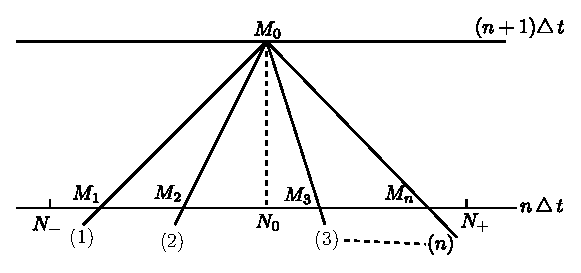
\includegraphics{figures/fig52-8.8.eps}
\caption{}\label{c8:fig8.8}
\end{figure}

We\pageoriginale choose a grid such that all the characteristics
through $M_\circ = (i\Delta x, (n+1)\Delta t)$ meet the line $n\Delta
t$ between $(i-1)\Delta x$ and $(i+1) \Delta x$. These two nodes have
been denoted by $N_-$ and $N_+$. The points where the characteristics
$(1), \ldots, (n)$ meet $n\Delta t$ are denoted by $M_1, \ldots M_n$,
respectively. Finally $N_\circ = (i\Delta x, \; n\Delta t)$.  

From the relation (\ref{eq8.53}), we write the approximate scheme
\begin{equation*}
p^T_k (U(M_\circ) - U(M_k)) = 0, \quad 1 \leq k \leq n . \tag{8.54}\label{eq8.54}
\end{equation*}
To compute $U(M_k)$, we use linear interpolation between $N_\circ$ and $N_+$ or between $N_\circ$ and $N_-$ according as $\lambda_k$ is $< 0$ or $> 0$. Thus we get $n$ equations for the $n$-components of $U(M_\circ)$ and we can solve this, in principle. This generalises the SNG-scheme.

\begin{remark}\label{chap8:rem8.6}
If we use quadratic interpolation between $N_-$, $N_\circ$ and $N_+$ we  get an analogue of the Lax-Wendroff scheme. 
\end{remark}

The stability condition is the same as condition (\ref{eq8.51}). The interpretation of this condition is that $[M_1, M_n] \subset \left[ N_- , N_+ \right]$ got from the Courant-Friedrichs-Lewy convergence condition, viz., the exact domain of dependence must lie within the approximate\pageoriginale domain of depnedence. Again to get condition (\ref{eq8.51}) we take the case for each characteristic and choose the strongest inequality amongst them.

\section{Non-linear systems-method of characteristics}\label{chap8:sec8.10}

If we have a pure dependence on $U$ of the matrix $A$ i.e. $A = A(U)$, we generalise the method of characteristics. The approximation of the equation (\ref{eq8.53}) will have to be centred between $M_\circ$ and $M_k$ for each $k$. We write
\begin{equation*}
\frac{p^T_k (U(M_k)) + p^T_k (U(M_\circ))}{2} (U(M_\circ ) - U(M_k)) = 0. 
\tag{8.55}\label{eq8.55}
\end{equation*}
and 
\begin{equation*}
M_k N_\circ = \frac{\Delta t}{2} [\lambda_k (U(M_\circ)) +\lambda_k(U(M_k))]. \tag{8.56}\label{eq8.56}
\end{equation*}

The unknowns are $x_k$, the abscissa of $M_k$, which can be got from the evaluation of $M_k N_\circ$, and also the $n$-components of $U(M_\circ)$ occurring in equation (\ref{eq8.55}).

We usually solve the system (\ref{eq8.55}) - (\ref{eq8.56}) by iterative methods. We assume $U^\circ (M_\circ)$ to start with. We assume all values  at level $n\Delta t$. Then setting 
\begin{equation*}
\left. 
\begin{aligned}
\lambda^{(\nu)}_k & = \frac{1}{2} (\lambda_k (U^{(\nu)} (M_\circ)) + \lambda_k (U(M^{(\nu)}_k))) \\
p^{T(\nu)}_k & = \frac{1}{2} (p^T_k (U^{(\nu)} (M_\circ)) + p^T_k (U(M^{(\nu)}_k)))
\end{aligned}
\right\}\tag{8.57}\label{eq8.57}
\end{equation*}
the iterative method could be 
\begin{equation*}
\left. 
\begin{aligned}
& M^{(\nu+1)}_k N_\circ = \lambda^{(\nu)}_k \Delta t.\\
&  p^{T(\nu)} _k (U^{(\nu+1)} (M_\circ) - U(M^{(\nu+1)}_k)) =0 . 
\end{aligned}
\right\}\tag{8.58}\label{eq8.58}
\end{equation*}
Now we use this to get $U^{(\nu+1)} (M_\circ)$ and $M^{(\nu+1)}_k N_\circ$. Thus we can again get $\lambda^{(\nu+1)}_k$ and $p^{T(\nu+1)}_k$ and proceed.

The\pageoriginale convergence of these iterations depends upon the nature of the non-linearity but is usually valid for small enough $\Delta t$. 

\begin{remark}\label{chap8:rem8.7}
When $n=2$, and when we have one positive and one negative eigenvalue, we can modify the method of characteristics.
\end{remark}

We fix a $\Delta x$ and draw both the characteristics through  each
point $i\Delta x$. Through the intersections of these we draw two more
and so on. (Cf. Fig. \ref{c8:fig8.9}). 

\begin{figure}[H]
\centering
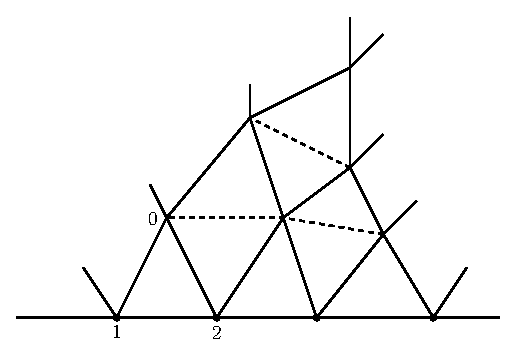
\includegraphics{figures/fig52-8.9.eps}
\caption{}\label{c8:fig8.9}
\end{figure}

If $U^T = (u,v)$, then the unknowns at $0$, are its coordinates $(x,t)$ and the values of $u$ and $v$. Then we use the following set of equations to obtain these values. 
\begin{align*}
\frac{x_\circ - x_1}{t_\circ - t_1} & = \frac{\lambda_1 (0) + \lambda_1(1)}{2} \tag{8.59}\label{eq8.59} \\
\frac{x_\circ - x_2}{t_\circ t_2} & = \frac{\lambda_2 (0) + \lambda_2 (2)}{2}  \tag{8.60} \label{eq8.60}
\end{align*}
\begin{align*}
\frac{1}{2} (p^T_1(0)  + P^T_1(1)). (U(0) - U(1)) = 0,
\tag{8.61}\label{eq8.61}\\ 
\frac{1}{2} (p^T_2 (0) + p^T_2 (2)). (U(0) - U(2)) = 0
\tag{8.62}\label{eq8.62} 
\end{align*}

We solve these, step by step at each node. Note that the nodes no longer form a regular mesh if $A$ is not constant. 

It is\pageoriginale this form of the method of characteristics which has been widely used in supersonic flow calculation. Its main advantage is that it does not need interpolation of the values of $u$ and $v$ which might be inaccurate.

\medskip
\noindent{\textbf{REFERENCES: }} Apart from the references cited in
the text, the reader could also look at the following papers: Lax
\cite{key21}. Lax and Wendroff \cite{key23, key24}, Boris and Book
\cite{key4}, Hirt \cite{key15}, Hoskin \cite{key16}, Kot \cite{key18},
Kasahara \cite{key17} and Gourlay and Morris \cite{key13}.
